\documentclass[letterpaper,final,12pt,reqno]{amsart}

\usepackage[total={6.3in,9.2in},top=1.1in,left=1.1in]{geometry}

\usepackage{times,bm,bbm,empheq,fancyvrb,graphicx,amsthm,amssymb}
\usepackage[dvipsnames]{xcolor}
\usepackage{longtable}
\usepackage{booktabs}

\usepackage{tabto}
\TabPositions{1.5cm}

\usepackage{tikz}
\usetikzlibrary{decorations.pathreplacing}

\usepackage{float}

% hyperref should be the last package we load
\usepackage[pdftex,
colorlinks=true,
plainpages=false, % only if colorlinks=true
linkcolor=blue,   % ...
citecolor=Red,    % ...
urlcolor=black    % ...
]{hyperref}

\renewcommand{\baselinestretch}{1.05}

\allowdisplaybreaks[1]  % allow display breaks in align environments, if they avoid major underfulls

\newtheoremstyle{cstyle}% name
  {5pt}% space above
  {5pt}% space below
  {\itshape}% body font
  {}% indent amount
  {\itshape}% theorem head font
  {.}% punctuation after theorem head
  {.5em}% space after theorem head
  {\thmname{#1}\thmnumber{ #2}\thmnote{ (#3)}}% theorem head spec
\theoremstyle{cstyle}

\newtheorem{theorem}{Theorem}
\newtheorem{lemma}[theorem]{Lemma}
\newtheorem{assumptions}[theorem]{Assumptions}

\newtheoremstyle{cstyle*}% name
  {5pt}% space above
  {5pt}% space below
  {\itshape}% body font
  {}% indent amount
  {\itshape}% theorem head font
  {.}% punctuation after theorem head
  {.5em}% space after theorem head
  {\thmname{#1}}% theorem head spec
\theoremstyle{cstyle*}
\newtheorem{assumptions*}{Assumptions}

\newtheoremstyle{dstyle}% name
  {5pt}% space above
  {5pt}% space below
  {}%{\itshape}% body font
  {}% indent amount
  {\itshape}% theorem head font
  {.}% punctuation after theorem head
  {.5em}% space after theorem head
  {\thmname{#1}\thmnumber{ #2}\thmnote{ (#3)}}% theorem head spec
\theoremstyle{dstyle}

\newtheorem{definition}[theorem]{Definition}
\newtheorem{example}[theorem]{Example}

%% numbering
\numberwithin{equation}{section}
%\numberwithin{figure}{section}
%\numberwithin{table}{section}
%\numberwithin{theorem}{section}

\newcommand{\eps}{\epsilon}

\newcommand{\RR}{\mathbb{R}}
\newcommand{\ZZ}{\mathbb{Z}}

\newcommand{\grad}{\nabla}
\newcommand{\Div}{\nabla\cdot}
\newcommand{\trace}{\operatorname{tr}}

\newcommand{\hbn}{\hat{\mathbf{n}}}

\newcommand{\bb}{\mathbf{b}}
\newcommand{\be}{\mathbf{e}}
\newcommand{\bbf}{\mathbf{f}}
\newcommand{\bg}{\mathbf{g}}
\newcommand{\bn}{\mathbf{n}}
\newcommand{\br}{\mathbf{r}}
\newcommand{\bu}{\mathbf{u}}
\newcommand{\bv}{\mathbf{v}}
\newcommand{\bw}{\mathbf{w}}
\newcommand{\bx}{\mathbf{x}}
\newcommand{\by}{\mathbf{y}}
\newcommand{\bz}{\mathbf{z}}

\newcommand{\bF}{\mathbf{F}}
\newcommand{\bV}{\mathbf{V}}
\newcommand{\bX}{\mathbf{X}}

\newcommand{\bxi}{\bm{\xi}}
\newcommand{\bzero}{\bm{0}}

\newcommand{\cK}{\mathcal{K}}
\newcommand{\cV}{\mathcal{V}}

\newcommand{\rhoi}{\rho_{\text{i}}}

\newcommand{\ip}[2]{\left<#1,#2\right>}

\newcommand{\maxR}{R^{\bm{\oplus}}}
\newcommand{\minR}{R^{\bm{\ominus}}}
\newcommand{\iR}{R^{\bullet}}

\newcommand{\nn}{{\text{n}}}
\newcommand{\pp}{{\text{p}}}
\newcommand{\qq}{{\text{q}}}
\newcommand{\rr}{{\text{r}}}

\newcommand{\supp}{\operatorname{supp}}
\newcommand{\Span}{\operatorname{span}}


\begin{document}
\title[A linear model for the coupled equations of glacier evolution]{A linear model for the coupled equations \\ of glacier evolution}

\author{Ed Bueler}

\date{\today}

\begin{abstract} FIXME
\end{abstract}

\maketitle

%\tableofcontents

\thispagestyle{empty}
%\bigskip

\newfloat{pseudofloat}{t}{xyz}[section]
\floatname{pseudofloat}{Algorithm}


\section{Introduction} \label{sec:intro}

The main problem of glaciology is to determine how changes to the geometry of a glacier, especially the ice thickness and ice-covered area, are determined by the climate experienced by the glacier, especially the surface mass balance.

This problem is interesting mathematically because the nontrivial equations for the bulk ice are two-way coupled to the equation for surface changes.  Ignoring conservation of energy, as here in these notes, the bulk ice equations are the conservation laws of mass and momentum.  Assuming incompressibility, the system is the Stokes equations for a very-viscous fluid \cite{Elmanetal2014,GreveBlatter2009}, which determine ice velocity and pressure from ice geometry and boundary stress inputs.  Note that the Stokes equations involve no time derivatives.  On the other hand, surface changes are modeled by the surface kinematical equation, often called the kinematic boundary condition \cite{GreveBlatter2009}, involving both a time derivative of the ice surface elevation and the surface value of the ice velocity.  We see that the bulk ice velocity and surface kinematics are nontrivially-coupled because the ice geometry (e.g.~surface elevation) determines the domain on which the Stokes equations apply, while the surface kinematical equation includes the ice velocity as a source term, in addition to the climatically-generated surface mass balance.

The full, coupled model is both an inequality-constrained free-boundary problem \cite{JouvetBueler2012}, because ice thickness is necessarily nonnegative, and highly nonlinear because the viscosity of ice is strain-rate dependent (shear-thinning; see \cite{GreveBlatter2009}).  This full, coupled model has yet to be mathematically analyzed, although at least the Stokes problem for fixed ice geometry is known to be well-posed \cite{JouvetRappaz2011}.  Numerical methods for this problem are at an early stage of development; existing methods scale poorly and stability-limited explicit time steps are in standard use \cite{Bueler2022preprint}.

It therefore makes sense, especially when exploring numerical solution methods, to construct a simpler linear mathematical model, one which nonetheless has the essential bulk-to-surface coupling.  That is, we can write down a system of equations which contain some aspects of the actual glaciological problem, but not all of difficult aspects at once.  These notes construct such a model.

In Section \ref{sec:model} we propose continuum equations which start with a 3D, scalar, elliptic partial differential equation (PDE), simpler than the Stokes equations.  We then couple a top-surface equation analogous to the steady-state of a glacier.  This 2D surface equation is scalar, like the surface kinematical equation, and the coupling has the character of the glacier problem because the surface value of the 3D problem's solution is a term in the 2D surface equation.  Furthermore, in this simpler, linear model we are able to \emph{explicitly} form the coupling term as a linear integral operator with an exact kernel.

After presenting the linear model equations the analogy with the glacier problem is presented (Section \ref{sec:analogy}), after which we consider numerical solutions in Section \ref{sec:numerical}, and then conclude.


\section{Model equations} \label{sec:model}

Our simpler, linear model problem is a 2D equation, \eqref{eq:modelproblem} below, with both partial derivatives and integrals.  It is created from a notional surface process on the top of a 3D domain.  We start with the 3D problem.

For length $\ell>0$ and height $h>0$ given, construct the rectangular solid $\Lambda = (0,\ell)^2\times (0,h)$ in 3D.  Coordinates on $\Lambda$ are $x,y,z$, with $0<x,y<\ell$ and $0<z<h$.  We call the $z=0$ boundary the \emph{bottom} and the $z=h$ boundary the \emph{top}, and the remaining boundaries the \emph{sides}.

Let $g(x,y)$ be a given function on the top, defined for $x,y \in (0,\ell)^2$.  Consider the following 3D Laplace equation problem, on $\Lambda$, for scalar solution $u(x,y,z)$:
\begin{subequations}
\label{eq:laplaceproblem}
\begin{align}
\grad^2 u &= 0 & &\text{in } \Lambda = (0,\ell)^2\times (0,h), \label{eq:laplaceproblemA} \\
u &= 0 & &\text{on the bottom and sides}, \label{eq:laplaceproblemB} \\
\frac{\partial u}{\partial z} &= g & &\text{on the top $z=h$}. \label{eq:laplaceproblemC}
\end{align}
\end{subequations}
Note that $\frac{\partial u}{\partial n}=\frac{\partial u}{\partial z}$ is the outward-normal derivative on top of $\Lambda$, so the input $g$ is the non-homogeneous Neumann condition in this 3D problem.  See Figure \ref{fig:laplaceproblem}.

\begin{figure}[ht]
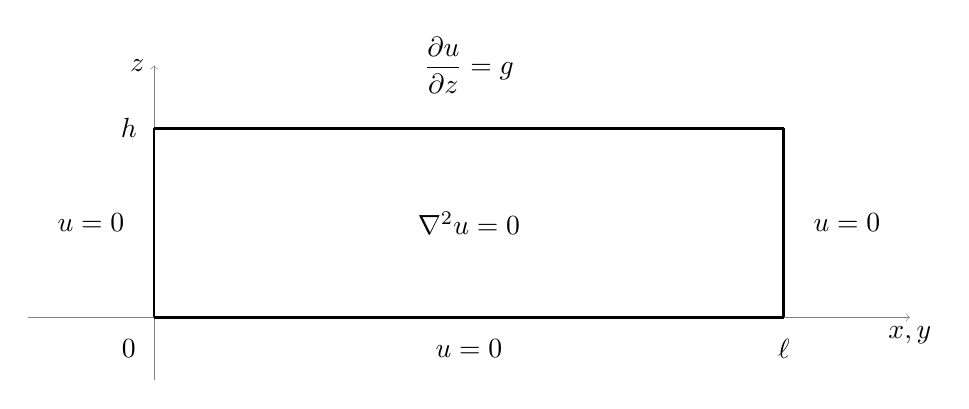
\begin{tikzpicture}[scale=8.0]
  % axes; x,y are horizontal and z is vertical
  \draw[->,gray,very thin] (-0.2,0.0) -- (1.2,0.0) node[below,black] {$x,y$};
  \draw[->,gray,very thin] (0.0,-0.1) -- (0.0,0.4) node[left,black] {$z$};
  % R = (0,L)^2
  \node at (-0.04,-0.05) {$0$};
  \node at (1.0,-0.05) {$\ell$};
  \node at (-0.04,0.3) {$h$};
  \draw[line width=1.0pt] (0.0,0.0) -- (0.0,0.3);
  \draw[line width=1.0pt] (1.0,0.0) -- (1.0,0.3);
  \draw[line width=1.0pt] (0.0,0.0) -- (1.0,0.0);
  \draw[line width=1.0pt] (0.0,0.3) -- (1.0,0.3);
  % equation and boundary conditions
  \node at (0.5,0.15) {$\grad^2 u = 0$};
  \node at (0.5,-0.05) {$u=0$};
  \node at (0.5,0.4) {$\displaystyle \frac{\partial u}{\partial z} = g$};
  \node at (-0.1,0.15) {$u=0$};
  \node at (1.1,0.15) {$u=0$};
\end{tikzpicture}
\caption{3D problem \eqref{eq:laplaceproblem} defines $u(x,y,z)$, for given Neumann condition $g(x,y)$.}
\label{fig:laplaceproblem}
\end{figure}

It is well-known that Laplace equation problem \eqref{eq:laplaceproblem} has a unique solution if $g$ is minimally well-behaved \cite{Elmanetal2014,Evans2010}.  The problem has a mixture of Dirichlet (bottom and sides) and Neumann (top) boundary conditions; the fact that Dirichlet conditions apply on a positive-measure part of the boundary of $\Lambda$ implies uniqueness.

Therefore it is reasonable to talk about \emph{the} solution $u$ of \eqref{eq:laplaceproblem}, as a function of the given top-surface Neumann data $g$.  In particular we define a map from $g$ to the top-surface solution values, the trace $u$ on the top \cite{Evans2010}.  Scaling by the parameter $h>0$, for reasons explained later, this defines a linear \emph{Neumann-to-Dirichlet map},
\begin{equation}
N_h : \, g(x,y) \, \mapsto \, \frac{1}{h} u(x,y,h).  \label{eq:ntod}
\end{equation}

As shown in the Appendix, a separation of variables argument allows us to express this map as an integral against a known kernel $K_h$, namely
\begin{equation}
(N_h g)(x,y) = \frac{1}{h} u(x,y,h) = \int_0^\ell \int_0^\ell K_h(x,y;\xi,\eta)\, g(\xi,\eta)\,d\xi\,d\eta  \label{eq:ntodformula}
\end{equation}
where
\begin{equation}
K_h(x,y;\xi,\eta) = \sum_{j=1}^\infty \sum_{k=1}^\infty \Phi\left(\frac{\pi \sqrt{j^2+k^2}\,h}{\ell}\right) \, \varphi_{jk}(x,y) \, \varphi_{jk}(\xi,\eta), \label{eq:kernelformula}
\end{equation}
with $\Phi(x)=\tanh(x)/x$ and $\varphi_{jk}(x,y) = (2/\ell) \sin(j\pi x/\ell) \sin(k\pi x/\ell)$; see equations \eqref{eq:app:laplaceproblemsoln} and \eqref{eq:app:kernelformula}.

Let $\Omega = (0,\ell)^2$.  As sketched in the Appendix, it follows from \eqref{eq:kernelformula} that
\begin{equation}
N_h g \to g  \label{eq:ntodasymptotic}
\end{equation}
for $g\in L^2(\Omega)$ as $h\to 0$.  That is, $N_h \to I$ in the strong sense as the aspect ratio of the 3D domain $\Lambda$ shrinks to zero (while keeping the horizontal dimension $\ell$ fixed).  Informal reasoning directly about problem \eqref{eq:laplaceproblem} will also lead to this conclusion.

Finally we can present our actual model problem.  Suppose that the ``$g$'' in problem \eqref{eq:laplaceproblem} is a function $s(x,y)$ which solves a ``surface process'' equation.  The surface equation is coupled to \eqref{eq:laplaceproblem}.  Adding an extra leading-order term using $\eps \ge 0$, the surface equation is
\begin{equation}
-\eps \grad^2 s + \frac{1}{h} u|_{z=h} = f,  \label{eq:premodelproblem}
\end{equation}
on the 2D domain $\Omega = (0,\ell)^2$, for a given source term $f(x,y)$.  To be clear, the ``$u$'' in \eqref{eq:premodelproblem} is the solution of \eqref{eq:laplaceproblem} in the case that $g=s$.

To fully define the model problem we add homogeneous Dirichlet boundary conditions for $s$ along $\partial \Omega$.  Furthermore, with our above definition of $N_h$, we may rewrite \eqref{eq:premodelproblem} as
\begin{equation}
-\eps \grad^2 s + N_h s = f.  \label{eq:modelproblem}
\end{equation}
Thus we understand the model problem to be a 2D integro-differential equation for $s$, given the source term $f(x,y)$, with homogeneous Dirichlet boundary conditions.  See Figure \ref{fig:modelproblem}.

\begin{figure}
\begin{tikzpicture}[scale=5.0]
  % axes
  \draw[->,gray,very thin] (-0.2,0.0) -- (1.2,0.0) node[below,black] {$x$};
  \draw[->,gray,very thin] (0.0,-0.2) -- (0.0,1.2) node[left,black] {$y$};
  % R = (0,L)^2
  \node at (-0.04,-0.05) {$0$};
  \node at (1.0,-0.05) {$\ell$};
  \node at (-0.04,1.0) {$\ell$};
  \draw[line width=1.0pt] (0.0,0.0) -- (0.0,1.0);
  \draw[line width=1.0pt] (1.0,0.0) -- (1.0,1.0);
  \draw[line width=1.0pt] (0.0,0.0) -- (1.0,0.0);
  \draw[line width=1.0pt] (0.0,1.0) -- (1.0,1.0);
  % equation and boundary conditions
  \node at (0.5,0.5) {$\displaystyle -\eps \grad^2 s + N_h s = f$};
  \node at (0.5,-0.1) {$s=0$};
  \node at (0.5,1.1) {$s=0$};
  \node at (-0.2,0.5) {$s=0$};
  \node at (1.2,0.5) {$s=0$};
\end{tikzpicture}
\caption{Model problem \eqref{eq:modelproblem} on $\Omega = (0,\ell)^2$.}
\label{fig:modelproblem}
\end{figure}


\section{Analogy with the steady and implicit-step glacier problems} \label{sec:analogy}

FIXME two-column analogy

FIXME briefly consider alternative model has ``$N_h \grad s$'' instead of $N_h s$, in some form?


\section{On multigrid solutions of \eqref{eq:modelproblem}} \label{sec:numerical}

FIXME \cite{Briggsetal2000,Bueler2021,Trottenbergetal2001} for multigrid

FIXME seek smoothers which can handle the $N_h$ integral operator

\section{Discussion and Conclusion} \label{sec:conclusion}

FIXME \cite{Girouardetal2022} show that the Neumann-to-Dirichlet map $\mathcal{N}:\frac{\partial u}{\partial n}|_{\partial} \mapsto u|_{\partial}$ along the \emph{entire} boundary of a 3D domain $\Lambda \subset \RR^3$ is very close to $|\grad_{\partial}|^{-1}$ where $|\grad_{\partial}| = \sqrt{-\grad_{\partial}^2}$ is the square root of the positive boundary Laplacian $-\grad_{\partial}^2$; they are identical only when $\Omega$ is a 3D sphere, which is not true here

\bibliography{model}
\bibliographystyle{siam}


\appendix
\section{Integral operator kernel for problem \eqref{eq:laplaceproblem}}

In this Appendix we give an explicit formula for the solution of the 3D Laplace equation problem \eqref{eq:laplaceproblem}, as illustrated in Figure \ref{fig:laplaceproblem}.  Formula \eqref{eq:app:laplaceproblemsoln} below is a Fourier sine series coming from a classical separation-of-variables type solution.  (A closed, non-series form may exist but it is not known to the author.)  The goal here is to derive kernel formula \eqref{eq:kernelformula}, the kernel of the Neumann-to-Dirichlet operator $N_h$, in a verifiable manner.

Consider the orthogonal set $\left\{\,\sin(j\pi x/\ell)\,\right\}_{j=1}^\infty$, a basis of $L^2(0,\ell)$.  Recall the following formulas:
    $$\int_0^\ell \sin(j\pi x/\ell) \sin(k\pi x/\ell)\,dx = \begin{cases} 0, & j \ne k \\ \ell/2, & j=k \end{cases}.$$
Fourier sine series follow.  In terms of orthonormal functions, if $f \in L^2(0,\ell)$ then
    $$f(x) = \sum_{j=1}^\infty c_j\, \sqrt{\frac{2}{\ell}} \sin(j\pi x/\ell) \quad \iff \quad c_j = \sqrt{\frac{2}{\ell}} \int_0^\ell f(x) \sin(j\pi x/\ell)\,dx.$$

Now consider the 2D domain $\Omega = (0,\ell)^2$ and define
    $$\varphi_{jk}(x,y) = \frac{2}{\ell} \sin(j\pi x/\ell) \sin(k\pi y/\ell).$$
For $j,k \in \ZZ$ these functions form an orthonormal (ON) basis in $L^2(\Omega)$, and furthermore $\varphi_{jk}(0,y)=\varphi_{jk}(\ell,y)=\varphi_{jk}(x,0)=\varphi_{jk}(x,\ell)=0$; they are zero on $\partial\Omega$.  We also see they are eigenfunctions of the Laplacian:
    $$\left(\frac{\partial^2}{\partial x^2} + \frac{\partial^2}{\partial y^2}\right) \varphi_{jk}(x,y) = - \frac{\pi^2 (j^2+k^2)}{\ell^2}\, \varphi_{jk}(x,y).$$
Again Fourier series formulas follow; if $g\in L^2(\Omega)$ then
    $$g(x,y) = \sum_{j=1}^\infty \sum_{k=1}^\infty c_{jk} \varphi_{jk}(x,y) \quad \iff \quad c_{jk} = \int_0^\ell \int_0^\ell g(x,y) \varphi_{jk}(x,y)\,dx\,dy.$$
The completeness of the set $\left\{\varphi_{jk}(x,y)\right\}_{j,k=1}^\infty$ is expressed by the Dirac delta function:
\begin{equation}
    \delta_{x,y}(\xi,\eta) = \sum_{j=1}^\infty \sum_{k=1}^\infty \varphi_{jk}(x,y) \, \varphi_{jk}(\xi,\eta). \label{eq:app:diracdelta}
\end{equation}

On the other hand, it is easily checked that for each pair $j,k \in \ZZ$ the modal function
    $$\sinh(\sqrt{j^2+k^2}\, \pi z/\ell) \, \varphi_{jk}(x,y)$$
solves equations \eqref{eq:laplaceproblemA} and \eqref{eq:laplaceproblemB}, that is, it solves the homogeneous parts of that problem.  By linearity this sum also solves equations \eqref{eq:laplaceproblemA} and \eqref{eq:laplaceproblemB}:
    $$u(x,y,z) = \sum_{j=1}^\infty \sum_{k=1}^\infty a_{jk} \sinh(\sqrt{j^2+k^2}\, \pi z/\ell)\, \varphi_{jk}(x,y),$$
assuming the coefficients $a_{jk}$ are appropriately summable.  We next seek to satisfy condition \eqref{eq:laplaceproblemC} for a given $g(x,y)$.  Note
    $$\frac{\partial u}{\partial z}(x,y,h) = \sum_{j=1}^\infty \sum_{k=1}^\infty a_{jk}\,\frac{\sqrt{j^2+k^2}\, \pi}{\ell} \cosh(\sqrt{j^2+k^2}\, \pi h/\ell) \, \varphi_{jk}(x,y)$$
It follows from uniqueness of coefficients, i.e.~orthogonality, that
    $$g(x,y) = \frac{\partial u}{\partial z}(x,y,h) \qquad \iff \qquad a_{jk} = \frac{\ell}{\pi \sqrt{j^2+k^2}\, \cosh(\sqrt{j^2+k^2}\, \pi h/\ell)} \,c_{jk}$$
where $c_{jk}$ are computed from $g(x,y)$ by the integral formula above.  Thus we may write a Fourier sine series solution of problem \eqref{eq:laplaceproblem}:
\begin{align}
u(x,y,z) &= \sum_{j=1}^\infty \sum_{k=1}^\infty \frac{\ell}{\pi \sqrt{j^2+k^2}\, \cosh(\sqrt{j^2+k^2}\, \pi h/\ell)} \,c_{jk} \, \sinh(\sqrt{j^2+k^2}\, \pi z/\ell) \,\varphi_{jk}(x,y) \notag \\
         &= \sum_{j=1}^\infty \sum_{k=1}^\infty \frac{\ell}{\pi \sqrt{j^2+k^2}\, \cosh(\sqrt{j^2+k^2}\, \pi h/\ell)} \,\left(\int_0^\ell \int_0^\ell g(\xi,\eta) \varphi_{jk}(\xi,\eta)\,d\xi\,d\eta\right) \notag \\
         &\qquad\qquad\qquad \cdot \sinh(\sqrt{j^2+k^2}\, \pi z/\ell) \, \varphi_{jk}(x,y). \label{eq:app:laplaceproblemsoln}
\end{align}

A formal simplification occurs if we evaluate at the surface and divide by $h$:
\begin{equation*}
\frac{1}{h} u(x,y,h) = \sum_{j=1}^\infty \sum_{k=1}^\infty \Phi\left(\frac{\pi \sqrt{j^2+k^2}\,h}{\ell}\right) \,\left(\int_0^\ell \int_0^\ell g(\xi,\eta) \varphi_{jk}(\xi,\eta)\,d\xi\,d\eta\right) \varphi_{jk}(x,y),
\end{equation*}
where
    $$\Phi(w) = \frac{\tanh(w)}{w}.$$
The function $\Phi$, sometimes called the ``$\operatorname{tanhc}$'' function,\footnote{See \href{https://en.wikipedia.org/wiki/Tanhc_function}{\texttt{en.wikipedia.org/wiki/Tanhc\_function}}.} is smooth on the real line and it satisfies $\Phi(0)=1$ and $\Phi'(0)=0$.  It has decay rate $\Phi(w) = O(w^{-1})$ as $w \to +\infty$.

Recalling that $(N_h g)(x,y) = h^{-1} u(x,y,h)$, by changing order of integration we have the following integral formula for the scaled, top-surface Neumann-to-Dirichlet $N_h$:
    $$(N_h g)(x,y) = \int_0^\ell \int_0^\ell K_h(x,y;\xi,\eta)\, g(\xi,\eta)\,d\xi\,d\eta$$
where
\begin{equation}
K_h(x,y;\xi,\eta) = \sum_{j=1}^\infty \sum_{k=1}^\infty \Phi\left(\frac{\pi \sqrt{j^2+k^2}\,h}{\ell}\right) \, \varphi_{jk}(x,y) \, \varphi_{jk}(\xi,\eta). \label{eq:app:kernelformula}
\end{equation}
This justifies kernel formula \eqref{eq:kernelformula} in the main text.

The decay of $\Phi(w)$ mentioned above, namely $\Phi(w) = O(w^{-1})$, implies that the eigenvalues of $N_h$ are $O((j^2+k^2)^{-1/2})$ as $j,k \to+\infty$.  Such decay is expected because the eigenvalues of the inverse of $N_h$, the Dirichlet-to-Neumann map, are known to go to infinity at the same rate as the square-root of the Laplacian \cite{Girouardetal2022}.  Observe that $N_h$ is a symmetric, compact operator \cite{Evans2010} on $L^2(\Omega)$.

As the aspect ratio $h/\ell$ goes to zero, observe that more and more modes $j,k$ correspond to small inputs $w=\pi \sqrt{j^2+k^2}\,h/\ell \ll 1$ going into $\Phi(w)$ in formula \eqref{eq:app:kernelformula}.  But $\Phi(w)\approx 1$ for such modes, since $\Phi(0)=1$ and $\Phi'(0)=0$.  Comparing the Dirac delta function \eqref{eq:app:diracdelta} to \eqref{eq:app:kernelformula}, we see that in the small aspect limit $K_h(x,y;\cdot,\cdot) \approx \delta_{x,y}(\cdot,\cdot)$.  (This requires well-behaved, smooth $g$ with a spectrum dominated by low frequencies.)  In fact, a standard Hilbert space argument shows that $N_h \to I$ as $h\to 0$, in the strong sense that $N_h g \to g$ in $L^2(\Omega)$.
\end{document}
